\section{Requisitos gerais}

Para o desenvolvimento de um sistema complexo como o proposto, faz-se necessário levantar requisitos de projeto mínimos, visando a utilidade, a eficiência e a acessibilidade disponibilizadas para o usuário. Dados a motivação e o objetivo do trabalho, temos os seguintes requisitos gerais:

\begin{enumerate}

	\item Ter uma maneira acessível e eficiente de ler códigos de barra: decidiu-se pelo uso de smartphones Android, a variação de smartphone mais utilizada. Além disso, se houver necessidade de que a OM possua celulares próprios para o controle de material que não o dos militares responsáveis por essa tarefa, tais smartphones têm menor custo, facilitando uma possível compra;

	\item Centralizar a informação de todos os materiais: um dos desafios atuais no controle dos materiais é a compilação das informações. Com a quantidade de papel envolvida, proveniente de anotações de várias pessoas diferentes vistoriando seções da OM, a compilação fica susceptível a erros humanos, seja por interpretação ou falta de atenção. O sistema deve ser capaz de fazer a compilação por si só; e
    
    \item Facilitar a geração de relatórios: novamente, a compilação das informações exige juntar as entradas de uma planilha, escrevendo uma a uma. O sistema deve ser capaz de gerar tal informação com as informações já centralizadas.
    
\end{enumerate}

\section{Especificações adicionais}

Complementando os requisitos levantados, há ainda as seguintes informações sobre os códigos de barra:

\begin{itemize}

	\item Cada material possui um código de barras único, mesmo que seja idêntico a outro material (duas cadeiras de escritório do mesmo modelo possuem códigos diferentes, por exemplo), e o código de barras é traduzido exatamente para o número identificador do material, conforme a Figura \ref{projfig01} abaixo.
    
    \begin{figure}[ht!]
        \centering
        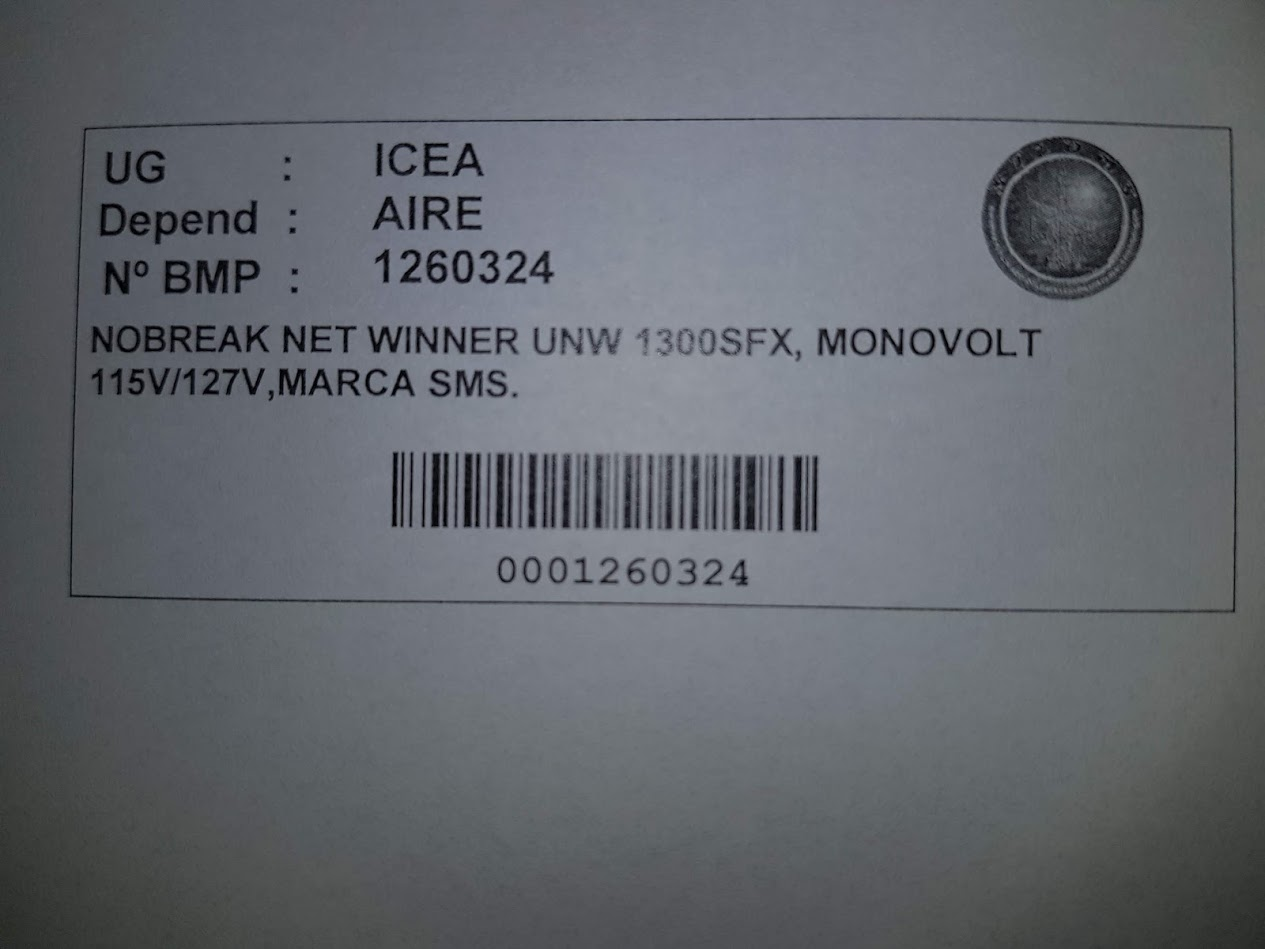
\includegraphics[width=0.75\textwidth]{Cap2/etiqueta}
        \caption{Modelo de etiqueta de material.}
        \label{projfig01}
    \end{figure}
    
    Pode-se ver que há também a informação da OM e da seção na etiqueta (respectivamente UG e Depend), além de uma breve descrição do material e de seu número identificador único.
    
    \item Cada OM possui um código identificador, assim como cada seção de cada OM.
    
\end{itemize}

\section{Decisões de programação}

\subsection{Programação do aplicativo}
Como o sistema operacional (SO) escolhido para os celulares foi o Android, havia a escolha entre Java e Kotlin, ambas linguagens aceitas pelo próprio Google (mantenedor do SO) como linguagens oficiais para programação em Android. Escolheu-se Kotlin pelas seguintes razões:

\begin{enumerate}

	\item Sintaxe: Kotlin foi construída com base no que os usuários de Java queriam de uma linguagem de programação. O resultado é uma linguagem mais atraente e simples de entender;
    
	\item Concisão: a linguagem reduz drasticamente a quantidade de \textit{boilerplate code}, isto é, seções de código que devem ser incluídas em muitos lugares com pouca ou nenhuma alteração, o que é bastante recorrente em Java;
    
    \item Interoperabilidade: a linguagem é mais recente que Java, e portanto a quantidade de bibliotecas produzidas para ela é bem menor. Porém, ela executa usando o mesmo ``motor'' que Java, o JVM, o que torna as duas linguagens completamente interoperáveis entre si;
    
    \item Segurança: a linguagem foi estruturada para evitar ao máximo a ocorrência \textit{exceptions} (erros durante a execução dos programas), principalmente um dos erros mais comuns de Java, o de ponteiro nulo.
    
\end{enumerate}

Kotlin é uma linguagem bem recente, a versão atual é 1.2.50. Para aprender a programar nessa linguagem, foram usados a documentação oficial da própria linguagem, o curso \cite{kotlinbeginners} para o básico da sintaxe e o curso \cite{kotlinandroid} para a programação própria do Android.

A versão mínima escolhida do Android que aceita o aplicativo é a versão 4.0.3 (Ice Cream Sandwich). Dessa forma, praticamente todos os dispositivos em circulação no mercado atualmente são abrangidos.

\subsection{Programação do banco de dados}

Integrar um sistema novo ou criar uma funcionalidade nova para o SILOMS exigiria muito mais tempo, principalmente devido a questões burocráticas. Com isso, foi decidido criar um sistema complementar ao SILOMS, que utilize dados dele e seja um servidor para todos os usuários do aplicativo desenvolvido. Escolheu-se criar uma API REST utilizando Node.js como \textit{back-end} do servidor (através das bibliotecas Loopback e Swagger) e MongoDB como fonte de dados.

Montar uma API REST foi a melhor opção encontrada para um servidor remoto de dados que alimenta um aplicativo Android, pois facilita a integração do banco de dados com o aplicativo e ainda permite que uma possível futura integração ao SILOMS ocorra facilmente, bastando apenas escrever as funções REST para o SILOMS servir como fonte de dados.

A escolha do Loopback é baseada na simplicidade: a biblioteca cria facilmente as rotas e comandos necessários para o funcionamento completo de uma estrutura CRUD (\textit{\textbf{C}reate, \textbf{R}ead, \textbf{U}pdate and \textbf{D}elete}), além de facilitar a integração com a fonte de dados e fornecer um sistema de autenticação. O Swagger cria uma interface gráfica para o servidor, permitindo o \textit{debug} visual das funções.

Simplicidade também foi o motivo da escolha do MongoDB. Os dados são armazenados em coleções, usando uma notação bastante semelhante ao JSON (\textit{JavaScript Object Notation}). Tal ordenação e classificação é bem próxima de uma \textit{array} de objetos em linguagens orientadas a objeto, o que facilita a combinação das duas formas quando se exporta ou importa dados.

Outro ponto importante a ser citado se refere ao requisito geral 3. Usar uma API REST em Node.js abre caminho para fazer uma interface gráfica de usuário (GUI) para solicitar o arquivo de relatório. Neste momento ainda não foi decidido quais bibliotecas usar para criar a GUI.
